\section{Mesh Nodes and Elements}
\label{sec:entities}

These routines describe and retreive the finite element mesh for this
computation.  A \term{mesh}, from the framework's perspective, is a list of
elements, nodes, and other data that describes the computational domain.
The FEM framework provides extensive support for creating, manipulating,
and partitioning meshes. 

A \term{serial mesh} consists of a single large piece.  It's usually
easiest to read and write serial meshes to existing, non-parallel file formats,
and it can be easier to manipulate serial meshes.  By contrast, a 
\term{parallel mesh} consists
of several pieces, called \term{chunks} or partitions.  Different processors
can work on different pieces of a parallel mesh, so most of the computation
is done using parallel meshes.  A simple program might create or read in a
single serial mesh in init, get a local chunk of the 
partitioned\footnote{The framework uses the excellent graph partitioning
package Metis.}
mesh in driver, and work on that chunk for the rest of the program.  
A more complex program might set an initial mesh in init; then get, 
work on, reassemble and repartition the mesh several times in driver 
via \kw{FEM\_Update\_mesh}.

\subsection{Mesh Entity Types}
A mesh consists of \term{entities}, such as nodes and elements.
Entities always have a \term{local number}, which is just the entities'
current index in its array.  Entites may also have a \term{global number}, 
which is the entity's index in the unpartitioned serial mesh.
Entities have data values called \term{attributes}.
For example, the location of each node might be called the 
``location'' attribute of the ``node'' entity type.  Attributes are
always stored in regular arrays indexed by the entity's local number.
This table lists the different attributes that can be read or
written for each type of entity.

A \term{shared entity} is a boundary entitity that two or more chunks 
can both update---currently, only nodes can be shared.  Shared nodes
are mixed in with regular nodes, and the framework currently provides
no way to identify which nodes are shared.

A \term{ghost entity} is a boundary entity that is asymmetrically shared---one
side provides values for the ghost from one of its real entities, 
and the other sides accept read-only copies of these values.
Ghosts are described in more detail in Section~\ref{sec:ghost},
and can be accessed by adding the constant \kw{FEM\_GHOST} to 
the corresponding real entity's type.

The different kinds of entities are described in the following sections.

\begin{center}
\begin{tabular}{|l|l|}\hline
Real Entity & Ghost Entity \\ \hline
\kw{FEM\_NODE} & \kw{FEM\_GHOST}+\kw{FEM\_NODE} \\ \hline
\kw{FEM\_ELEM}+$elType$ & \kw{FEM\_GHOST}+\kw{FEM\_ELEM}+$elType$ \\ \hline
\kw{FEM\_SPARSE}+$sparseType$ & \kw{FEM\_GHOST}+\kw{FEM\_SPARSE}+$sparseType$ \\ \hline
\end{tabular}
\end{center}



\subsubsection{Nodes}
\kw{FEM\_NODE} is the entity code for nodes, the simplest kind of entity.  
A node is a single point in the domain, and elements are defined by their nodes.
Nodes can have the following attributes:

\begin{itemize}
\item \kw{FEM\_DATA}+$tag$  Uninterpreted user data, which might
    include material properties, boundary conditions, flags, etc.
    User data can have any data type and width.
    $tag$ can be any number from 0 to one billion---it allows you
    to register several data fields with a single entity.

\item \kw{FEM\_GLOBALNO}  Global node numbers. Always a 1-wide index type.

\item \kw{FEM\_SYMMETRIES} Symmetries that apply to this node.  
    Always a 1-wide \kw{FEM\_BYTE}.

\item \kw{FEM\_NODE\_PRIMARY}  Marker indicating that this chunk is responsible 
    for this node.  Every node is primary in exactly one chunk.
    This attribute is always a 1-wide \kw{FEM\_BYTE} containing 0 or 1.

% \item \kw{FEM\_COORD}  Optional coordinates for this node.
\end{itemize}


\subsubsection{Elements}
\kw{FEM\_ELEM}+$elType$ is the entity code for one kind of element.
$elType$ is a small, user-defined value that uniquely identifies 
this element type.  Like nodes, elements can have the attributes
\kw{FEM\_DATA}+$tag$, \kw{FEM\_GLOBALNO}, or \kw{FEM\_SYMMETRIES};
but every element type must have this attribute:

\begin{itemize}
\item \kw{FEM\_CONN} Lists the numbers of the nodes around this element. 
    See the description in the ghost section for special ghost connectivity.
    Always an index type--\kw{FEM\_INDEX\_0} for C-style 0-based node indexing,
    or \kw{FEM\_INDEX\_1} for Fortran-style 1-based node indexing.
\end{itemize}


\subsubsection{Sparse Elements}
\kw{FEM\_SPARSE}+$sparseType$ is the entity code for one kind of sparse element.
Again, $sparseType$ is a small, user-defined unique value.
The only difference between ordinary elements and sparse elements 
regards partitioning.  Ignoring ghosts, ordinary elements are never duplicated---each
element is sent to its own chunk.  Sparse elements may be duplicated,
and are always dependent on some other entity for their partitioning.
Sparse elements have all the attributes of ordinary elements:
\kw{FEM\_DATA}+$tag$, \kw{FEM\_GLOBALNO}, \kw{FEM\_SYMMETRIES},
and \kw{FEM\_CONN}, as well as the special attribute \kw{FEM\_SPARSE\_ELEM}.

Without the \kw{FEM\_SPARSE\_ELEM} attribute, a sparse element will 
be copied to every chunk that contains all the sparse element's nodes.  
This is useful for things like node-associated boundary conditions, 
where the sparse element connectivity might list the nodes with boundary
conditions, and the sparse element data might list the boundary condition values.

The \kw{FEM\_SPARSE\_ELEM} attribute lists the ordinary element each 
sparse element should be partitioned with.  This attribute consists of 
pairs ($elType$,$elNum$), indicating that this sparse element
should be sent to wherever the $elNum$'th \kw{FEM\_ELEM}+$elType$ 
is partitioned.


\begin{itemize}
\item \kw{FEM\_SPARSE\_ELEM} Lists the element we should be partitioned with.
    The width of this attribute is always 2, and the data type must
    be an index type--\kw{FEM\_INDEX\_0} or \kw{FEM\_INDEX\_1}.
% & \kw{FEM\_COORD} & Optional coordinates for this node.
\end{itemize}



\subsection{Mesh Entity Manipulation}


\prototype{FEM\_Mesh\_default\_read}
\function{int FEM\_Mesh\_default\_read(void);}
\function{INTEGER function :: FEM\_Mesh\_default\_read()}

Return the default reading mesh.  This routine is valid:

\begin{itemize}
\item From \kw{driver()}, to return the partitioned mesh.
\item During your FEM\_Update\_mesh routine, to return the assembled mesh.
\item Anytime after a call to FEM\_Mesh\_set\_default\_read.
\end{itemize}

\prototype{FEM\_Mesh\_default\_write}
\function{int FEM\_Mesh\_default\_write(void);}
\function{INTEGER function :: FEM\_Mesh\_default\_write()}

Return the default writing mesh.  This routine is valid:

\begin{itemize}
\item From \kw{init()}, to change the new serial mesh.
\item From \kw{driver()}, to change the new partitioned mesh.
\item During your FEM\_Update\_mesh routine, to change the new serial mesh.
\item Anytime after a call to FEM\_Mesh\_set\_default\_write.
\end{itemize}


\prototype{FEM\_Mesh\_get\_length}  
\function{int FEM\_Mesh\_get\_length(int mesh,int entity);}
\function{INTEGER function :: FEM\_Mesh\_get\_length(mesh,entity)}
  \args{INTEGER, INTENT(IN) :: mesh,entity }

Return the number of \uw{entity}s that exist in this \uw{mesh}.

This call can be used with any entity.
For example, to get the number of nodes,
  \begin{alltt}
      nNodes=FEM\_Mesh\_get\_length(\uw{mesh},\kw{FEM\_NODE})
  \end{alltt}
To get the number of ghost nodes, 
  \begin{alltt}
      nGhostNodes=FEM\_Mesh\_get\_length(\uw{mesh},\kw{FEM\_GHOST}+\kw{FEM\_NODE})
  \end{alltt}
To get the number of real elements of type 2,
  \begin{alltt}
  	nElem=FEM\_Mesh\_get\_length(\uw{mesh},\kw{FEM\_ELEM}+2)
  \end{alltt}


\prototype{FEM\_Mesh\_data}  
\function{void FEM\_Mesh\_data(int mesh,int entity,int attr,
        void *data, int first, int length, int datatype,int width);}
\function{SUBROUTINE FEM\_Mesh\_data(mesh,entity,attr,data,first,length,datatype,width)}
  \args{INTEGER, INTENT(IN) :: mesh,entity,attr,first,length,datatype,width}
  \args{datatype, intent(inout) :: data(width,length) }

This is the one routine for getting or setting entity's attributes 
on the mesh.  

\begin{itemize}
\item \uw{mesh} A FEM mesh object.  Depending on whether this is
   a reading or writing mesh, this routine reads from or writes to
   the data array you pass in.

\item \uw{entity} A FEM entity code, for example \kw{FEM\_NODE} or
   \kw{FEM\_GHOST}+\kw{FEM\_ELEM}+1.

\item \uw{attr} A FEM attribute code, for example \kw{FEM\_DATA}+$tag$
   or \kw{FEM\_CONN}.  
 
\item \uw{data} The user data to get or set.  Each row of this array consists
  of \uw{width} values, and contains the data values of the attribute for the
  corresponding entity.  This data must be formatted as one of:
  \begin{alltt}
      datatype :: data(width,length)
      datatype :: data(width*length)
  \end{alltt}

\item \uw{first} The first entity to affect.  In C, this is normally 0;
  in Fortran, this is normally 1.

\item \uw{length} The number of entities to affect.  The entities
  affected are thus those numbered from \uw{first} to \uw{first}+\uw{length}-1.
  For now, \uw{length} must be either 1, to touch a single entity; or
  else the total number of entities--that is, FEM\_Mesh\_get\_length(mesh,entity).

\item \uw{datatype} The data type stored in this attribute.  This
  is one of the standard FEM data types \kw{FEM\_BYTE}, \kw{FEM\_INT}, 
  \kw{FEM\_FLOAT}, or \kw{FEM\_DOUBLE}; or else the C-style 0-based
  index type \kw{FEM\_INDEX\_0} or the Fortran-style 1-based index type
  \kw{FEM\_INDEX\_1}. Alternatively, the equivalent types \kw{IDXL\_BYTE}, \kw{IDXL\_INT},
\kw{IDXL\_FLOAT}, \kw{IDXL\_DOUBLE}, \kw{IDXL\_INDEX\_0}, or \kw{IDXL\_INDEX\_1} may be used.

\item \uw{width} The number of data items per entity. 

\end{itemize}

For example, to set the element connectivity, which is stored as 
3 integer node indices in \uw{nodes}, you would:

  \begin{alltt}
/* C version */
   int *nodes=new int[3*nElems];
   ... fill out nodes ...
   FEM\_Mesh\_data(mesh,FEM\_ELEM+1,FEM\_CONN, nodes, 0,nElems, FEM\_INDEX\_0, 3);
   ... continue to use or delete nodes ...
   
! F90 version
   ALLOCATE(nodes(3,nElems))
   ... fill out nodes ...
   CALL FEM\_Mesh\_data(mesh,FEM\_ELEM+1,FEM\_CONN, nodes, 1,nElems, FEM\_INDEX\_1, 3)
   ... continue to use or delete nodes ...
  \end{alltt}

To add a new node property with 2 double-precision numbers 
from an array \uw{mat} (containing, for example,
material properties), you would first pick an unused
user data "tag", for example 13, and:

  \begin{alltt}
/* C version */
   double *mat=new double[2*nNodes];
   ...
   FEM\_Mesh\_data(mesh,FEM\_NODE, FEM\_DATA+13, mat, 0,nNodes, FEM\_DOUBLE, 2);
   
! F90 version
   ALLOCATE(mat(2,nNodes))
   CALL FEM\_Mesh\_data(mesh,FEM\_NODE,FEM\_DATA+13, mat, 1,nNodes, FEM\_DOUBLE, 2)
  \end{alltt}


\subsection{Entity Inquiry}

\prototype{FEM\_Mesh\_get\_width}  
\function{int FEM\_Mesh\_get\_width(int mesh,int entity,int attr);}
\function{INTEGER function :: FEM\_Mesh\_get\_width(mesh,entity,attr)}
  \args{INTEGER, INTENT(IN) :: mesh,entity,attr }

Return the width of the attribute \uw{attr} of \uw{entity} of \uw{mesh}.
This is the value previously passed as ``width'' to FEM\_Mesh\_data.


\prototype{FEM\_Mesh\_get\_datatype}  
\function{int FEM\_Mesh\_get\_datatype(int mesh,int entity,int attr);}
\function{INTEGER function :: FEM\_Mesh\_get\_datatype(mesh,entity,attr)}
  \args{INTEGER, INTENT(IN) :: mesh,entity,attr }

Return the FEM data type of the attribute \uw{attr} of \uw{entity} of \uw{mesh}.
This is the value previously passed as ``datatype'' to FEM\_Mesh\_data.


\prototype{FEM\_Mesh\_get\_entities}  
\function{int FEM\_Mesh\_get\_entities(int mesh,int *entities);}
\function{INTEGER function :: FEM\_Mesh\_get\_entities(mesh,entities)}
  \args{INTEGER, INTENT(IN) :: mesh}
  \args{INTEGER, INTENT(OUT) :: entities(:) }

Extract an array of the different entities present in this mesh.
Returns the number of entity types present.  The \uw{entities}
array must be big enough to hold all the different entities in
the mesh.

For example, a simple mesh might have two entity types:
FEM\_NODE and FEM\_ELEM+1.


\prototype{FEM\_Mesh\_get\_attributes}  
\function{int FEM\_Mesh\_get\_attributes(int mesh,int entity,int *attributes);}
\function{INTEGER function :: FEM\_Mesh\_get\_attributes(mesh,entity,attributes)}
  \args{INTEGER, INTENT(IN) :: mesh, entity}
  \args{INTEGER, INTENT(OUT) :: attributes(:) }

Extract an array of the different attributes of this entity.
Returns the number of attribute types present.  The \uw{attributes}
array must be big enough to hold all the attributes.

For example, a simple element might have three attributes:
FEM\_CONN for node connectivity, FEM\_GLOBALNO for global element
numbers, and FEM\_DATA+7 for a material type.

\prototype{FEM\_Get\_*\_name}  
\function{const char *FEM\_Get\_entity\_name(int entity,char *storage);}
\function{const char *FEM\_Get\_attr\_name(int attr,char *storage);}
\function{const char *FEM\_Get\_datatype\_name(int datatype,char *storage);}

Return a human-readable name for this FEM entity, attribute, or datatype.
The \uw{storage} array must point to a buffer of at least 100 characters;
this array might be used as temporary space to store the returned string.

These routines are only available in C.


\subsection{Advanced Entity Manipulation}

\prototype{FEM\_Mesh\_data\_offset}  
\function{void FEM\_Mesh\_data\_offset(int mesh,int entity,int attr,
        void *data, int first, int length, int datatype,int width,
	int offsetBytes,int distanceBytes,int skewBytes);}
\function{SUBROUTINE FEM\_Mesh\_data\_offset(mesh,entity,attr,data,first,length,datatype,width,
	offsetBytes,distanceBytes,skewBytes)}
  \args{INTEGER, INTENT(IN) :: mesh,entity,attr,first,length,datatype,width}
  \args{INTEGER, INTENT(IN) :: offsetBytes,distanceBytes,skewBytes }
  \args{datatype, intent(inout) :: data(width,length) }

This routine is a more complicated version of FEM\_Mesh\_data.
It allows you to get or set a mesh field directly
from a user-defined structure.  See the documentation of
IDXL\_Layout\_offset in Section~\ref{sec:IDXLLayoutoffset}
for details on how to set offsetBytes, distanceBytes, and skewBytes.

\prototype{FEM\_Mesh\_data\_layout}
\function{
void FEM\_Mesh\_data\_layout(int mesh,int entity,int attr,
      void *data, int firstItem, int length, IDXL\_Layout\_t layout);
}
\function{SUBROUTINE FEM\_Mesh\_data\_layout(mesh,entity,attr,data,first,length,layout)}
  \args{INTEGER, INTENT(IN) :: mesh,entity,attr,first,length,layout}
  \args{INTEGER, INTENT(IN) :: layout}

This routine is a more complicated version of FEM\_Mesh\_data.
Like FEM\_Mesh\_data\_offset, it allows you to get or set a mesh
field directly from a user-defined structure; but this routine
expects the structure to be described by an IDXL\_Layout object.

%%%%%%%%%%%%%%%%%%%%%% Mesh Creation %%%%%%%%%%%%%%%%%%%%%%%%%%
\section{Meshes}
\label{sec:mesh}

A "mesh" is a collection of nodes and elements 
knit together in memory, as described in Section~\ref{sec:terminology}.
Meshes are always referred to by an integer that 
serves as a handle to the local mesh.

This section describes routines to manipulate entire meshes
at once: this includes calls to create and delete meshes,
read and write meshes,
partition and reassemble meshes, and send meshes between
processors.

Only a few of the mesh routines are collective; 
most of them only describe local data and hence 
operate independently on each chunk.


\subsection{Mesh Routines}

\prototype{FEM\_Mesh\_allocate}
\function{int FEM\_Mesh\_allocate(void);}
\function{INTEGER FUNCTION :: FEM\_Mesh\_allocate()}

Create a new local mesh object.  The mesh is initially empty,
but it is a setting mesh, so call FEM\_Mesh\_data 
to fill the mesh with data.


\prototype{FEM\_Mesh\_deallocate}
\function{int FEM\_Mesh\_deallocate(int mesh);}
\function{SUBROUTINE FEM\_Mesh\_deallocate(mesh)}
  \args{INTEGER, INTENT(IN) :: mesh}

Destroy this local mesh object, and its associated
data.


\prototype{FEM\_Mesh\_copy}
\function{int FEM\_Mesh\_copy(int mesh);}
\function{INTEGER FUNCTION FEM\_Mesh\_copy(mesh)}
  \args{INTEGER, INTENT(IN) :: mesh}

Create a new mesh object with a separate copy of the data 
stored in this old mesh object.


\prototype{FEM\_Mesh\_write}
\function{void FEM\_Mesh\_write(int mesh,const char *prefix,int partNo,int nParts);}
\function{SUBROUTINE FEM\_Mesh\_write(mesh,prefix,partNo,nParts)}
  \args{INTEGER, INTENT(IN) :: mesh}
  \args{INTEGER, INTENT(IN) :: partNo,nParts}
  \args{character (LEN=*), INTENT(IN) :: prefix}

Write this mesh to the file ``\uw{prefix}\_vp\uw{partNo}\_\uw{nParts}.dat''.

By convention, \uw{partNo} begins at 0; but no index conversion is
performed so you can assign any meaning to \uw{partNo} and \uw{nParts}.
In particular, this routine is not collective--you can read any
mesh from any processor.
For example, if \uw{prefix} is ``foo/bar'', the data for the 
first of 7 chunks would be stored in ``foo/bar\_vp0\_7.dat''
and could be read using FEM\_Mesh\_read('foo/bar',0,7).

Meshes are stored in a machine-portable format internal to FEM.
The format is currently ASCII based, but it is subject to change.
We strongly recommend using the FEM routines to read and write 
these files rather than trying to prepare or parse them yourself.


\prototype{FEM\_Mesh\_read}
\function{int FEM\_Mesh\_read(const char *prefix,int partNo,int nParts);}
\function{INTEGER FUNCTION :: FEM\_Mesh\_read(prefix,partNo,nParts)}
  \args{INTEGER, INTENT(IN) :: partNo,nParts}
  \args{character (LEN=*), INTENT(IN) :: prefix}

Read a new mesh from the file ``\uw{prefix}\_vp\uw{partNo}\_\uw{nParts}.dat''.
The new mesh begins in getting mode, so you can read the 
data out of the mesh using calls to FEM\_Mesh\_data.



\prototype{FEM\_Mesh\_broadcast}
  \function{int FEM\_Mesh\_broadcast(int mesh,int fromRank,FEM\_Comm\_t comm\_context);}
  \function{INTEGER FUNCTION :: FEM\_Mesh\_broadcast(mesh,fromRank,comm\_context)}
     \args{INTEGER, INTENT(IN) :: mesh,fromRank,comm\_context}

Take the mesh \uw{mesh} on processor \uw{fromRank} (normally 0), 
partition the mesh into one piece per processor (in the MPI communicator
\uw{comm\_context}, and return each processor its own piece 
of the partitioned mesh.  This call is collective, but only 
processor \uw{fromRank} needs to pass in a \uw{mesh}; the 
\uw{mesh} value is ignored on other processors.

For example, if rank 0 has a mesh named ``src'', we can 
partition src for all the processors by executing:
\begin{alltt}
  m=FEM_Mesh_broadcast(src,0,MPI_COMM_WORLD);
\end{alltt}

The new, partitioned mesh is in getting mode, so 
you can read the partitioned data using calls to FEM\_Mesh\_data.
This call does not affect \uw{mesh} in any way.

  
\prototype{FEM\_Mesh\_reduce}
  \function{int FEM\_Mesh\_reduce(int mesh,int toRank,FEM\_Comm\_t comm\_context);}
  \function{INTEGER FUNCTION :: FEM\_Mesh\_reduce(mesh,toRank,comm\_context);}
     \args{INTEGER, INTENT(IN) :: mesh,toRank,comm\_context}

This call is the reverse operation of FEM\_Mesh\_broadcast:
each processor passes in a mesh in \uw{mesh}, the mesh is 
assembled, and the function returns the assembled mesh
to processor \uw{toRank}.  This call is collective, but 
only processor \uw{toRank} is returned a mesh; all other
processors are returned the non-mesh value 0.

The new, reassembled mesh is in getting mode.
This call does not affect \uw{mesh}.


\subsection{Mesh Utility}

\prototype{FEM\_Mesh\_is\_get}
\function{int FEM\_Mesh\_is\_get(int mesh)}
\function{INTEGER FUNCTION :: FEM\_Mesh\_is\_get(mesh)}
  \args{INTEGER, INTENT(IN) :: mesh }

Return true if this mesh is in getting mode.
A getting mesh returns values to FEM\_Mesh\_data.

\prototype{FEM\_Mesh\_is\_set}
\function{int FEM\_Mesh\_is\_set(int mesh)}
\function{INTEGER FUNCTION :: FEM\_Mesh\_is\_set(mesh)}
  \args{INTEGER, INTENT(IN) :: mesh }

Return true if this mesh is in setting mode.
A setting mesh extracts values from FEM\_Mesh\_data.


\prototype{FEM\_Mesh\_become\_get}
\function{void FEM\_Mesh\_become\_get(int mesh)}
\function{SUBROUTINE :: FEM\_Mesh\_become\_get(mesh)}
  \args{INTEGER, INTENT(IN) :: mesh }

Put this mesh in getting mode, so you can read back
its values.

\prototype{FEM\_Mesh\_become\_set}
\function{void FEM\_Mesh\_become\_set(int mesh)}
\function{SUBROUTINE :: FEM\_Mesh\_become\_set(mesh)}
  \args{INTEGER, INTENT(IN) :: mesh }

Put this mesh in setting mode, so you can set its values.

\prototype{FEM\_Mesh\_print}
\function{void FEM\_Mesh\_print(int mesh);}
\function{SUBROUTINE FEM\_Mesh\_print(mesh)}
    \args{INTEGER, INTENT(IN) :: mesh}

Print out a text description of the nodes and elements 
of this mesh.


\subsection{Advanced Mesh Manipulation}

\prototype{FEM\_Mesh\_pup}
\function{typedef void (*FEM\_Userdata\_fn)(pup\_er p,void *data);}
\function{void FEM\_Mesh\_pup(int mesh,int pupTag,FEM\_Userdata\_fn fn,void *data);}
\function{SUBROUTINE myPupFn(p,data);}
   \args{INTEGER, INTENT(IN) :: p}
   \args{TYPE(myType) :: data}
\function{SUBROUTINE FEM\_Mesh\_pup(mesh,pupTag,myPupFn,data);}
   \args{INTEGER, INTENT(IN) :: mesh,pupTag}
   \args{SUBROUTINE :: myPupFn}
   \args{TYPE(myType) :: data}

Store \uw{data} with this \uw{mesh}.  \uw{data} is a struct or TYPE
with a pup function \uw{myPupFn}---see the TCharm manual for details 
on writing a pup function.
\uw{pupTag} is an integer used to distinguish different pieces of data
associated with this mesh.

When called on a setting mesh, this routine stores \uw{data};
when called on a getting mesh, this routine reads out \uw{data}.

\uw{data} will be associated with the mesh itself, not any 
entity in the mesh.  This makes it useful for storing shared
data, often simulation constants such as the timestep or material 
properties.  \uw{data} is made a part of the mesh, and it will be 
read and written, sent and received, partitioned and assembled
with the mesh.


\prototype{FEM\_Mesh\_send}
  \function{void FEM\_Mesh\_send(int mesh,int toRank,int tag,FEM\_Comm\_t comm\_context);}
  \function{SUBROUTINE FEM\_Mesh\_send(mesh,toRank,tag,comm)}
    \args{INTEGER, INTENT(IN) :: mesh,toRank,tag,comm}
  
  Send the mesh \uw{mesh} to the processor \uw{toRank}, using
  the MPI tag \uw{tag} and communicator \uw{comm\_context}.
  Tags are normally only needed if you plan to mix direct MPI
  calls with your FEM calls.
  
  This call does not affect \uw{mesh}.
  

\prototype{FEM\_Mesh\_recv}
  \function{int FEM\_Mesh\_recv(int fromRank,int tag,FEM\_Comm\_t comm\_context);}
  \function{INTEGER FUNCTION FEM\_Mesh\_recv(fromRank,tag,comm)}
    \args{INTEGER, INTENT(IN) :: fromRank,tag,comm}
  
  Receive a new mesh from the processor \uw{fromRank}, using
  the MPI tag \uw{tag} and communicator \uw{comm\_context}.
  You can also use the special values MPI\_ANY\_SOURCE as \uw{fromRank}
  to receive a mesh from any processor, or use
  MPI\_ANY\_TAG for \uw{tag} to match any tag.

  The new mesh is returned in getting mode.

\prototype{FEM\_Mesh\_partition}
  \function{void FEM\_Mesh\_partition(int mesh,int nParts,int *destMeshes);}
  \function{SUBROUTINE FEM\_Mesh\_partition(mesh,nParts,destMeshes)}
    \args{INTEGER, INTENT(IN) :: mesh,nParts}
    \args{INTEGER, INTENT(OUT) :: destMeshes(nParts)}

Divide \uw{mesh} into \uw{nParts} pieces, and store the pieces
into the array \uw{destMeshes}. 

The partitioned mesh is returned in getting mode.
This is a local call; FEM\_Mesh\_broadcast is the collective version.
This call does not affect the source mesh \uw{mesh}.

  
\prototype{FEM\_Mesh\_assemble}
  \function{int FEM\_Mesh\_assemble(int nParts,const int *srcMeshes);}
  \function{INTEGER FUNCTION FEM\_Mesh\_assemble(nParts,srcMeshes)}
    \args{INTEGER, INTENT(IN) :: nParts, srcMeshes(nParts)}

Assemble the \uw{nParts} meshes listed in \uw{srcMeshes} into
a single mesh.  Corresponding mesh pieces are matched using 
the attribute FEM\_GLOBALNO.  Specifically, if the value of 
the integer index attribute FEM\_GLOBALNO for an entity is $i$,
the entity will be given the number $i$ in the reassembled mesh.
If you do not set FEM\_GLOBALNO, the different pieces of the 
mesh will remain separate---even ``matching'' nodes will not be merged.

The assembled mesh is returned in getting mode.
This is a local call; FEM\_Mesh\_reduce is the collective version.
This call does not affect the source meshes.


\prototype{FEM\_Mesh\_copy\_globalno}
  \function{void FEM\_Mesh\_copy\_globalno(int src\_mesh,int dest\_mesh);}
  \function{SUBROUTINE FEM\_Mesh\_copy\_globalno(src\_mesh,dest\_mesh)}
    \args{INTEGER, INTENT(IN) :: src\_mesh,dest\_mesh}

Copy the FEM\_GLOBALNO attribute for all the entity types in 
\uw{src\_mesh} into all the matching types in \uw{dest\_mesh},
where the matching types exist.  This call is often used 
before an FEM\_Mesh\_assemble or FEM\_Mesh\_reduce to synchronize
global numbers before reassembly.


%%%%%%%%%%%%%%%%%%%%%% Ghosts %%%%%%%%%%%%%%%%%%%%%%%%%%

\section{Mesh Ghosts}
\label{sec:ghost}

A \term{ghost entity} is a local, read-only copy of a real entity
on another chunk. Ghosts are typically added to the boundary of a chunk to allow the real (non-ghost) elements at the boundary to access values across the processor boundary.  This makes a chunk ``feel'' as if it was part of a complete unpartitioned mesh; and can be useful with cell-centered methods, and in mesh modification.

\begin{figure}
\begin{center}
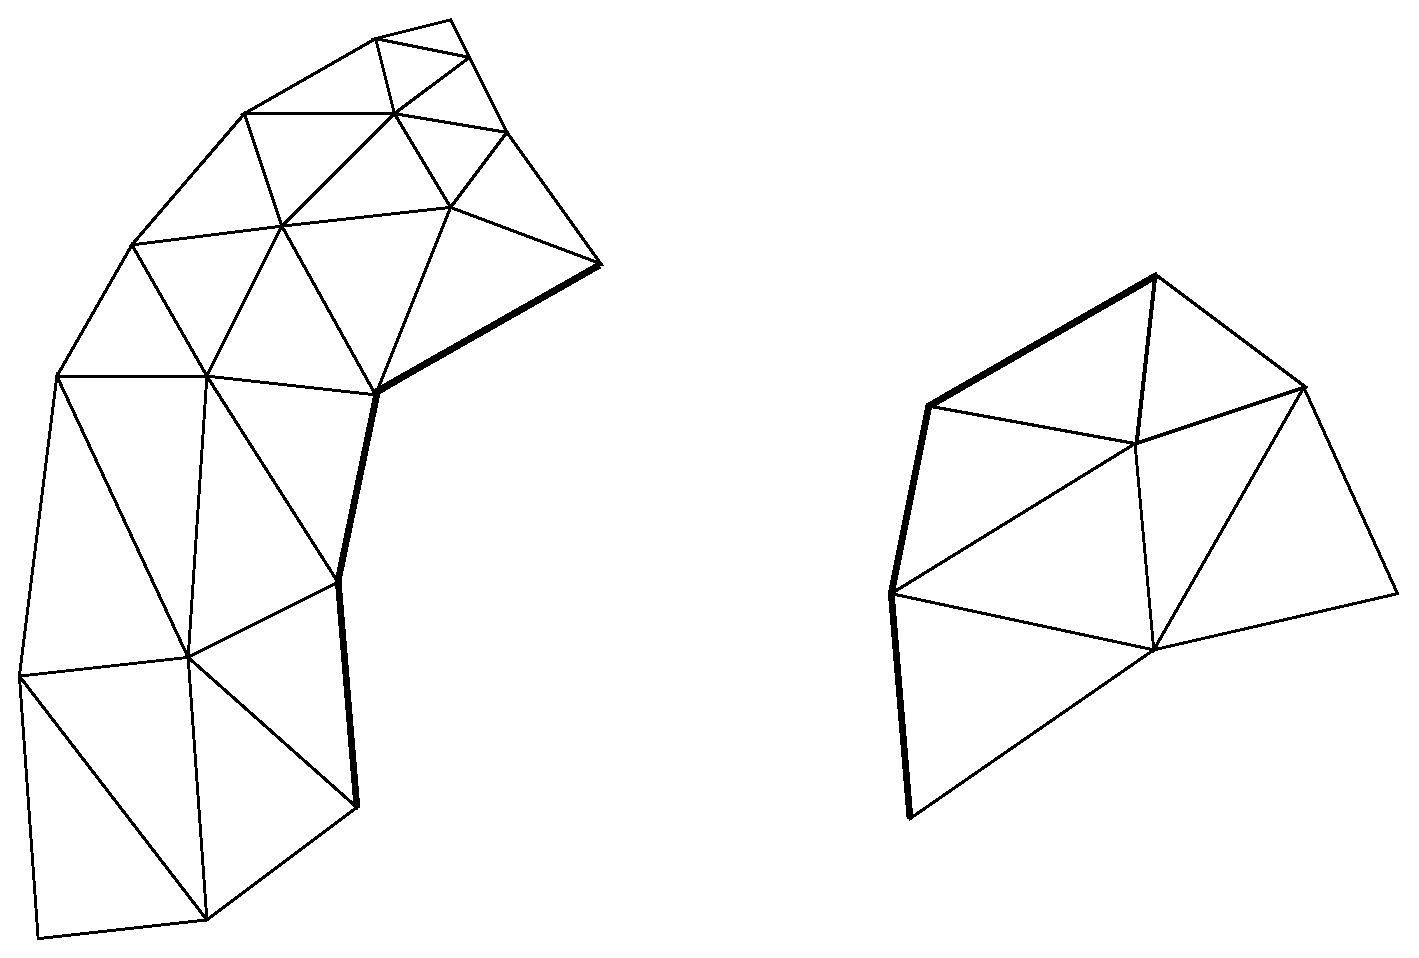
\includegraphics[width=1.5in]{fig/ghost_pre}
\end{center}
\caption{A small mesh partitioned into two pieces.}
\label{fig:ghostpre}

% \end{figure} \begin{figure} % Make sure these two figures don't get separated

\begin{center}
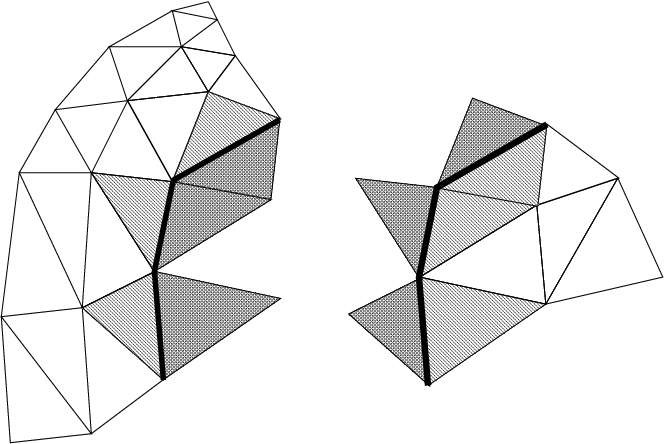
\includegraphics[width=1.5in]{fig/ghost_edge}
\end{center}
\caption{The same mesh with one layer of edge-adjacent ghosts.}
\label{fig:ghostedge}

% \end{figure} \begin{figure}

\begin{center}
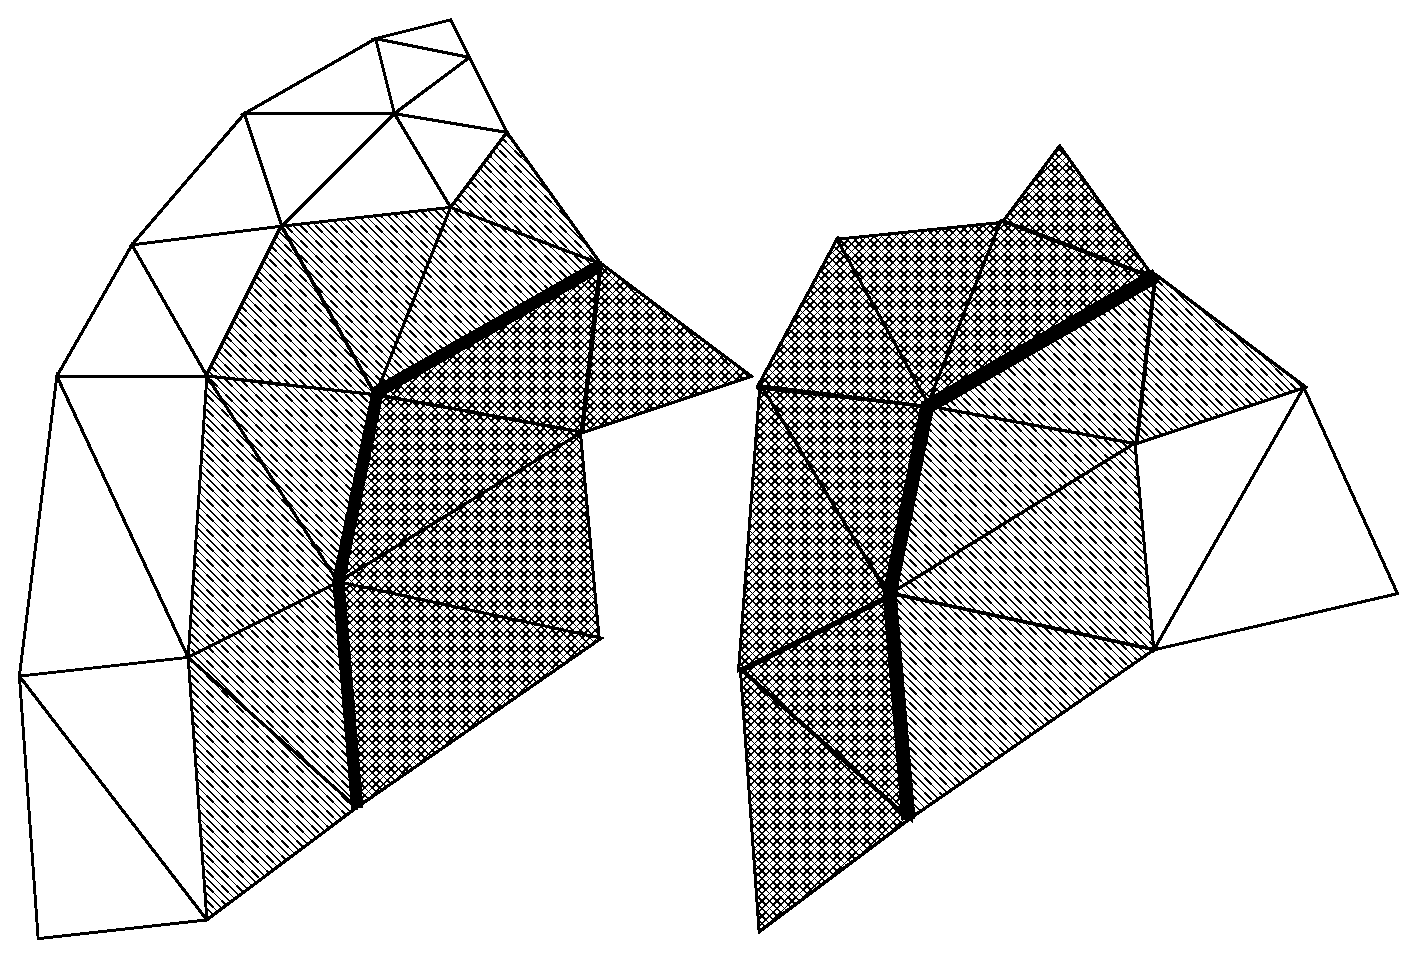
\includegraphics[width=1.5in]{fig/ghost_node}
\end{center}
\caption{The same mesh with one layer of node-adjacent ghosts.}
\label{fig:ghostnode}
\end{figure}


In Figure~\ref{fig:ghostpre}, we begin with a small mesh partitioned
into pieces on the left and right.  In Figure~\ref{fig:ghostedge},
we have added ghost elements (dark hashing) that share an edge with
adjacent real elements (light hatching).  In Figure~\ref{fig:ghostnode},
we add ghost elements that share at least one node with adjacent 
real elements.



\subsection{Ghost Numbering}
\label{sec:ghostnum}
Ghosts and real entities are stored by the framework
in separate lists---to access the ghost entity type, add \kw{FEM\_GHOST}
to the real entity's type.  For example, \kw{FEM\_GHOST}+\kw{FEM\_ELEM}+1 
lists the ghost elements for \uw{elType} 1.  To get the number 
of ghost nodes, you would call 
\kw{FEM\_Mesh\_get\_length}(\uw{mesh},\kw{FEM\_GHOST}+\kw{FEM\_NODE}).

\begin{figure}[h]
\begin{center}
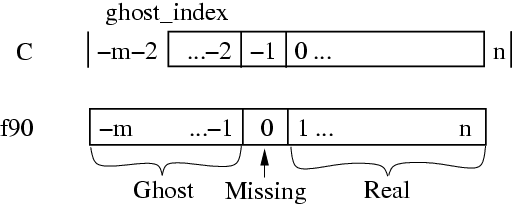
\includegraphics[width=4in]{fig/conn_indexing}
\end{center}
\caption{Node indices used in the element connectivity array.
There are $n$ real nodes and $m$ ghosts.}
\label{fig:connindexing}
\end{figure}

For real elements, the element connectivity always consists of real nodes.
But for ghost elements, the adjacent nodes may be missing, or may themselves
be ghosts.
Thus ghost element connectivity lists may include the invalid 
value -1 (in C) or 0 (in Fortran) to indicate that the corresponding 
node is not present; or may include values
less than this, which indicate the corresponding node is a ghost.
In C, ghost node $i$ is indicated by the value $-2-i$, while
in Fortran, ghost node $i$ is indicated by the value $-i$.  
This node indexing system is illustrated in Figure~\ref{fig:connindexing}, 
This indexing system is bizarre, but it allows us to keep
the real and ghost nodes clearly separate, while still
allowing real and ghost nodes to be added in increasing order
at both ends.

Since the C tests are complicated, in C we recommend using these macros:

\begin{itemize}
\item \kw{FEM\_Is\_ghost\_index}(i) returns true if $i$ represents a ghost node.
In Fortran, use the test $i$ .lt. $0$

\item \kw{FEM\_From\_ghost\_index}(i) returns the ghost node's index given its connectivity entry.
In Fortran, use the expression $-i$.

\item \kw{FEM\_To\_ghost\_index}(i) returns the connectivity entry for a given ghost node index.
In Fortran, again use the expression $-i$.
\end{itemize}

For example, a quadrilateral ghost element that is adjacent to, respectively, two real 
nodes 23 and 17, the tenth local ghost node, and one not-present node might have a 
connectivity entry of {23,17,-11,-1} (in C) or {23,17,-10,0} (in Fortran).

Applications may wish to use some other numbering,
such as by storing all the ghost nodes after all the real nodes.
The code to extract and renumber the connectivity of some 3-node triangles 
stored in FEM\_ELEM+2 would be:

\begin{alltt}
/* C version */
  int nReal=FEM\_Mesh\_get\_length(mesh,FEM\_ELEM+2);
  int nGhost=FEM\_Mesh\_get\_length(mesh,FEM\_GHOST+FEM\_ELEM+2);
  typedef int intTriplet[3];
  intTriplet *conn=new intTriplet[nReal+nGhost];
  /* Extract real triangles into conn[0..nReal-1] */
  FEM\_Mesh\_data(mesh,FEM\_ELEM+2,FEM\_CONN, &conn[0][0], 0,nReal, 3,FEM\_INDEX\_0);
  /* Extract ghost triangles into conn[nReal..nReal+nGhost-1] */
  FEM\_Mesh\_data(mesh,FEM\_GHOST+FEM\_ELEM+2,FEM\_CONN, &conn[nReal][0], 0,nGhost, 3,FEM\_INDEX\_0);
  
  /* Renumber the ghost triangle connectivity */
  for (int t=nReal;t<nReal+nGhost;t++)
    for (int i=0;i<3;i++) \{
      int in=conn[t][i]; /* uses FEM ghost node numbering */
      int out; /* uses application's ghost numbering */
      if (in==-1) \{ 
        out=some\_value\_for\_missing\_nodes; 
      \} else if (FEM\_Is\_ghost\_index(in)) \{
        out=first\_application\_ghost+FEM\_From\_ghost\_index(in);
      \} else /*regular real node*/ \{
        out=in;
      \}
      conn[t][i]=out;
    \}

! F90 version
  INTEGER, ALLOCATABLE :: conn(3,:)
  INTEGER :: nReal,nGhost,t,i,in,out
  nReal=FEM\_Mesh\_get\_length(mesh,FEM\_ELEM+2)
  nGhost=FEM\_Mesh\_get\_length(mesh,FEM\_GHOST+FEM\_ELEM+2)
  ALLOCATE(conn(3,nReal+nGhost))
  ! Extract real triangles into conn[1..nReal] 
  CALL FEM\_Mesh\_data(mesh,FEM\_ELEM+2,FEM\_CONN, conn, 1,nReal, 3,FEM\_INDEX\_1)
  ! Extract ghost triangles into conn[nReal+1..nReal+nGhost] 
  CALL FEM\_Mesh\_data(mesh,FEM\_GHOST+FEM\_ELEM+2,FEM\_CONN, conn(1,nReal+1), 1,nGhost, 3,FEM\_INDEX\_1)
  
  ! Renumber the ghost triangle connectivity 
  DO t=nReal+1,nReal+nGhost
    DO i=1,3
      in=conn(i,t) 
      IF (in .EQ. 0) out=some\_value\_for\_missing\_nodes
      IF (in .LT. 0) out=first\_application\_ghost-1+(-in)
      IF (in .GT. 0) out=in
      conn(i,t)=out
    END DO
  END DO
  
  
\end{alltt}



\subsection{Setting up the ghost layer}
The framework's ghost handling is element-centric. You specify which kinds of elements should be ghosts and how they connect by listing their faces before partitioning.  

\begin{itemize}
\item

\prototype{FEM\_Add\_ghost\_layer}
\function{void FEM\_Add\_ghost\_layer(int nodesPerFace,int doAddNodes);}
\function{SUBROUTINE FEM\_Add\_ghost\_layer(nodesPerFace,doAddNodes)}
  \args{INTEGER, INTENT(IN) :: nodesPerFace,doAddNodes}
This routine creates a new layer of ghosts around each FEM chunk. \kw{nodesPerFace} is the number of shared nodes that together form a ``face''. \kw{doAddNodes} specifies that you want ghost nodes around your ghost elements.  If \kw{doAddNodes} is 0, ghost elements will have invalid -1 (in C) or 0 (in Fortran) connectivity entries where there is no corresponding local node.

A face is an unordered ``tuple'' of nodes, and is an abstract way to describe which ghosts
your application needs---an element will be added to your chunk if it connects to at 
least one of your elements' faces.  For example, if you have a 3D, tetrahedral element that require ghosts 
on all 4 of its sides, this is equivalent to requiring ghosts of every element that shares all 3
nodes of one of your triangular faces, so for you a face is a 3-node triangle.  If you have a 2D shape
and want edge-adjacency, for you a face is a 2-node edge.  If you want node-adjacent ghosts,
a face is a single node.

Calling this routine several times creates several layers of ghost elements, and the different layers need not have the same parameters.

\item
\prototype{FEM\_Add\_ghost\_elem}
\function{void FEM\_Add\_ghost\_elem(int elType,int facesPerElem,const int *elem2face);}
\function{SUBROUTINE FEM\_Add\_ghost\_elem(elType,facesPerElem,elem2face)}
  \args{INTEGER, INTENT(IN) :: elType,facesPerElem}
  \args{INTEGER, INTENT(IN) :: elem2face(nodesPerFace,facesPerElem)}

This call is used to specify which type of element is to be added to the current ghost layer. \kw{facesPerElem} and \kw{elem2face} specify a mapping between each element and the surrounding faces.  The \kw{elem2face} table lists, for each face, the nodes of this element which form the face, specified as element-local numbers---indices into this element's connectivity entry. The \kw{elem2face} table should have nodesPerFace*facesPerElem entries, and no entry should be greater than nodePerEl for that element type.

Because all faces must take up the same space in the array,
\kw{elem2face} can include special indices--- -1 for C, 0 for Fortran---that indicate the
corresponding face is actually shorter than usual.  For example, if \kw{nodesPerFace} for this layer
is 4, for 4-node quadrilateral faces, you could set one entry in \kw{elem2face} to -1 to specify
this is a 3-node triangular face.  Faces of different lengths will never match, so this is just
a simple way to add ghosts from two kinds of faces at once.

\end{itemize}

The above two routines are always used together. For example, if your elements are 3-node triangles and you only require one shared node for inclusion in a single ghost layer, you would use:
\begin{alltt}
   FEM\_Add\_ghost\_layer(1,1); /* 1 node per face: node adjacency */
   const static int tri2node[]=\{0,1,2\};
   FEM\_Add\_ghost\_elem(0,3,tri2node); /* triangles are surrounded by 3 nodes */
\end{alltt}

If you require two shared nodes (a shared edge), the code will look like:
\begin{alltt}    
   FEM\_Add\_ghost\_layer(2,1); /* 2 nodes per face: edge adjacency */
   const static int tri2edge[]=\{0,1,  1,2,  2,0\};
   FEM\_Add\_ghost\_elem(0,3,tri2edge); /*triangles are surrounded by 3 edges */
\end{alltt}


\subsection{Symmetries and Ghosts--Geometric Layer}

The FEM framework can create ghosts not only of things that are on other 
processors, but also for various problem symmetries, like mirror reflection,
and various types of periodicities.  The interface for these ghosts is 
simple---you ask for the symmetries to be created, then you will get 
extra ghosts along each symmetry boundary.  The symmetry ghosts are
updated properly during any communication, even if the symmetry ghosts
are ghosts of real local elements from the same chunk.


\begin{figure}[h]
\begin{center}
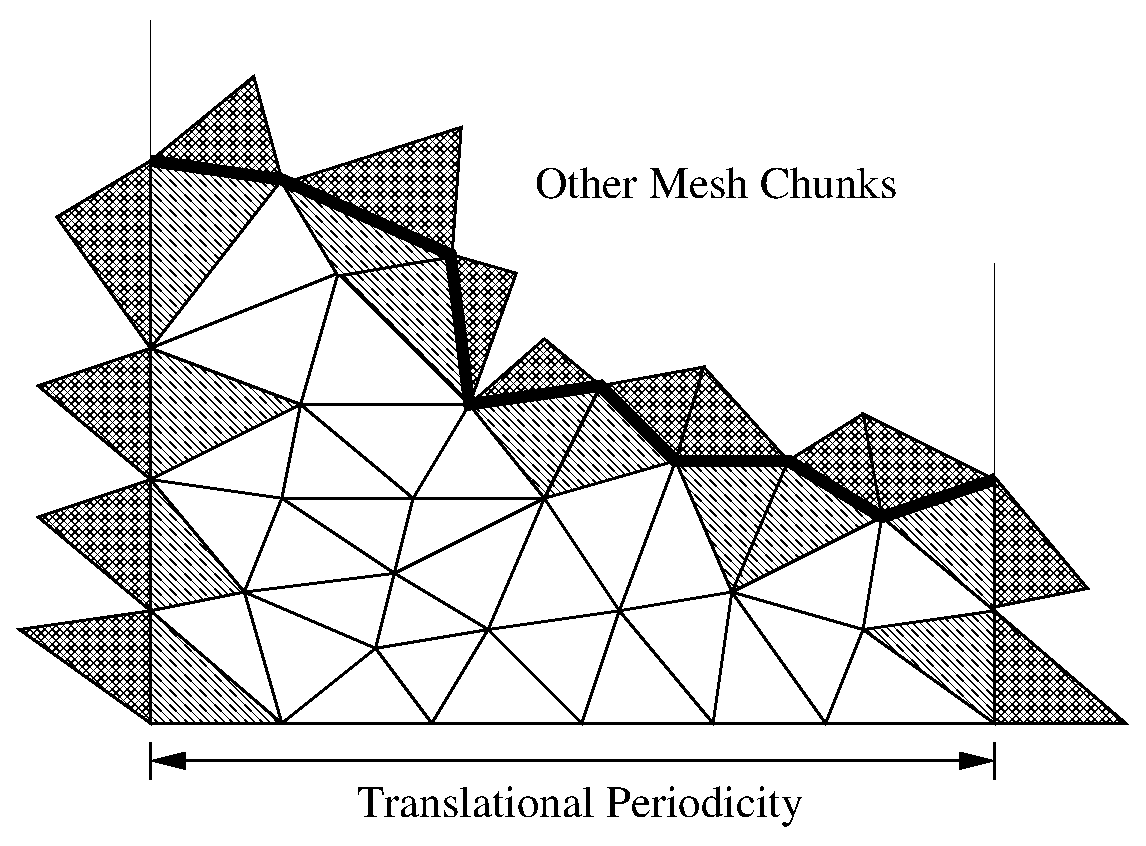
\includegraphics[width=3in]{fig/sym_ghost}
\end{center}
\caption{Illustrating symmetry ghost elements.}
\label{fig:symghost}
\end{figure}

Figure~\ref{fig:symghost} shows a chunk of a mesh for a 
rectangular domain with horizontal linear translational periodicity---that 
is, the domain repeats horizontally.
Symmetry ghosts lie along the left and right sides; ordinary cross-processor
parallel ghosts lie along the top edge where this chunk joins up with the
rest of the domain; and the external boundary along the bottom of the chunk
has no ghosts.



\prototype{FEM\_Add\_linear\_periodicity}
\function{void FEM\_Add\_linear\_periodicity(
        int nFaces,int nPer,
        const int *facesA,const int *facesB,
        int nNodes,const double *nodeLocs
        );}
\function{
SUBROUTINE FEM\_Add\_linear\_periodicity(nFaces,nPer,facesA,facesB,
                                nNodes,nodeLocs)}
  \args{INTEGER, INTENT(IN) :: nFaces, nPer, nNodes}
  \args{INTEGER, INTENT(IN) :: facesA(nPer,nFaces), facesB(nPer,nFaces)}
  \args{double precision, INTENT(IN) :: nodeLocs(3,nNodes)}

Make facesA and facesB match up under linear translation.
Each face of facesA must match up with exactly one face of
facesB, but both the faces and the nodes within a face can be
permuted in any order---the order is recovered by matching 3d locations
in the nodeLocs array.

This call can be repeated, for example if the domain is periodic along several
directions.  This call can only be issued from \kw{init()}.



\prototype{FEM\_Sym\_coordinates}
\function{void FEM\_Sym\_coordinates(int elTypeOrMinusOne,double *locs);}
\function{SUBROUTINE FEM\_Sym\_coordinates(elTypeOrZero,locs)}
  \args{INTEGER, INTENT(IN) :: elTypeOrZero}
  \args{double precision, intent(inout) :: locs(3,<number of items>)}

This call adjusts the 3d locations listed in \kw{locs} so they respect the symmetries
of their corresponding item.  If elTypeOrZero is an element type,
the locations are adjusted to match with the corresponding element;
if elTypeOrZero is zero, the locations are adjusted to match up with
the corresponding node.

This call is needed because symmetry ghost nodes and elements
initially have their original locations, which must be adjusted
to respect the symmetry boundaries.  Thus this call is needed
both for initial location data (e.g., from \kw{FEM\_Get\_node\_data})
as well as any communicated location data (e.g., from
\kw{FEM\_Update\_ghost\_field}).

This call can only be issued from \kw{driver()}.



\subsection{Advanced Symmetries and Ghosts--Lower Layer}

The geometric symmetry layer in the preceeding section is actually
a thin wrapper around this lower, more difficult to use layer.

\prototype{FEM\_Set\_sym\_nodes}
\function{void FEM\_Set\_sym\_nodes(const int *canon,const int *sym);}
\function{SUBROUTINE FEM\_Set\_sym\_nodes(canon,sym)}
  \args{INTEGER, INTENT(IN) :: canon(nNodes)}
  \args{INTEGER, INTENT(IN) :: sym(nNodes)}

This call describes all possible symmetries in an extremely terse format.
It can only be called from \kw{init()}.
The ``canonicalization array'' canon maps nodes to their canonical 
representative---if canon($i$)=canon($j$), nodes $i$ and $j$ are 
images of each other under some symmetry.  The sym array has bits set
for each symmetry boundary passing through a node.

For example, a 2d domain with 6 elements A, B, C, D, E, and F and 12 
nodes numbered 1-12 that is 
mirror-symmetric on the horizontal boundaries but periodic in the 
vertical boundaries would look like:

\begin{alltt}
   D^'|  D^ |  E^ |  F^ |  F^`
   -  1  -  2  -  3  -  4  -
   A' |  A  |  B  |  C  |  C`
   -  5  -  6  -  7  -  8  -
   D' |  D  |  E  |  F  |  F`
   -  9  - 10  -  11 -  12 -
   Av'|  Av |  Bv |  Cv |  Cv`

  v indicates the value has been shifted down (bottom boundary),
  ^ indicates the value has been shifted up (top boundary),
  ' indicates the value has been copied from the left (right boundary),
  ` indicates the value has been copied from the right (left boundary).
\end{alltt}

If we mark the left border with 1, the top with 2, the right with 4,
and the bottom with 8, this situation is indicated by topologically pasting the 
top row to the bottom row by setting their \kw{canon} entries equal, and 
marking each node with its symmetries.

\begin{center}
\begin{tabular}{|l|l|l|}\hline
  Node & \kw{canon} &  \kw{sym}              \\\hline
    1  &    1  &      3 (left + top)   \\
    2  &    2  &      2 (top)   \\
    3  &    3  &      2 (top)   \\
    4  &    4  &      6 (top + right)   \\
    5  &    5  &      1 (left)   \\
    6  &    6  &      0 (none)   \\
    7  &    7  &      0 (none)   \\
    8  &    8  &      4 (right)   \\
    9  &    1  &      9 (left+bottom)    \\
    10 &    2  &      8 (bottom)   \\
    11 &    3  &      8 (bottom)   \\
    12 &    4  &      12 (bottom+right)   \\
\hline
\end{tabular}
\end{center}


\prototype{FEM\_Get\_sym}
\function{void FEM\_Get\_sym(int elTypeOrMinusOne,int *destSym);}
\function{void FEM\_Get\_sym(elTypeOrZero,destSym);}
  \args{INTEGER, INTENT(IN) :: elTypeOrMinusOne }
  \args{INTEGER, INTENT(OUT) :: destSym(nItems)}

This call extracts the list of symmetry conditions that apply to 
an item type.  If elType is an element type, it returns the
symmetry conditions that apply to that element type; if elType is
-1 (zero for Fortran), it returns the symmetry conditions that apply
to the nodes.  Symmetry conditions are normally only nonzero
for ghost nodes and elements.


Mirror symmetry conditions are not yet supported, nor are
multiple layers of symmetry ghosts, but both should be easy to add
without changing this interface.

% FIXME: document these
% void FEM\_Set\_partition(int *elem2chunk)
% int FTN\_NAME(FEM\_GET\_COMM\_PARTNERS,fem\_get\_comm\_partners)(void)
% int FTN\_NAME(FEM\_GET\_COMM\_PARTNER,fem\_get\_comm\_partner)(int *partnerNo)
% int FTN\_NAME(FEM\_GET\_COMM\_COUNT,fem\_get\_comm\_count)(int *partnerNo)
% void FTN\_NAME(FEM\_GET\_COMM\_NODES,fem\_get\_comm\_nodes)(int *pNo,int *nodeNos)
% void FTN\_NAME(FEM\_GET\_ELEM\_NUMBERS,fem\_get\_elem\_numbers)(int *gNo)
% void fem\_get\_node\_numbers(int *gNo)





%%%%%%%%%%%%%%%%%%%%%% Old Mesh %%%%%%%%%%%%%%%%%%%%%%%%%%

\section{Older Mesh Routines}
These routines have a simpler, but less flexible interface
than the general routines described in Section~\ref{sec:entities}.  Because they are 
easy to implement in terms of the new routines, they will remain
part of the framework indefinitely.
These routines always use the default mesh, as returned by 
\kw{FEM\_Mesh\_default\_read} and \kw{FEM\_Mesh\_default\_write}.


\prototype{FEM\_Get/Set\_elem}
\function{void FEM\_Set\_elem(int elType,int  nEl,int  doublePerEl,int  nodePerEl);}
\function{void FEM\_Get\_elem(int elType,int *nEl,int *doublePerEl,int *nodePerEl);}
\function{SUBROUTINE FEM\_Set\_elem(elType,nEl,doublePerEl,nodePerEl)}
  \args{INTEGER, INTENT(IN)  :: elType,nEl,doublePerEl,nodePerEl}
\function{SUBROUTINE FEM\_Get\_elem(elType,nEl,doublePerEl,nodePerEl)}
  \args{INTEGER, INTENT(IN)  :: elType}
  \args{INTEGER, INTENT(OUT) :: nEl,doublePerEl,nodePerEl}

     Describe/retreive the number and type of elements.  \kw{ElType} is a
user-defined small, unique element type tag.  \kw{nEl} is the number of elements 
being registered.  \kw{doublesPerEl} and \kw{nodePerEl} are the number of doubles of user data, and nodes (respectively) associated with each element.

     \kw{doublePerEl} or \kw{nodePerEl} may be zero, indicating that no user
data or connectivity data (respectively) is associated with the element.

     You can make this and any other mesh setup calls in any order---there is no need 
to make them in linearly increasing order.  However, for a given type of element
\kw{FEM\_Set\_elem} must be called before setting that element's connectivity or data.


\prototype{FEM\_Get/Set\_elem\_conn}
\function{void FEM\_Set\_elem\_conn(int elType,const int *conn);}
\function{void FEM\_Get\_elem\_conn(int elType,int *conn);}
\function{SUBROUTINE FEM\_Set\_elem\_conn\_r(elType,conn)}
  \args{INTEGER, INTENT(IN)  :: elType}
  \args{INTEGER, INTENT(IN),  dimension(nodePerEl,nEl) :: conn}
\function{SUBROUTINE FEM\_Get\_elem\_conn\_r(elType,conn)}
  \args{INTEGER, INTENT(IN)  :: elType}
  \args{INTEGER, INTENT(OUT), dimension(nodePerEl,nEl) :: conn}
\function{SUBROUTINE FEM\_Set\_elem\_conn\_c(elType,conn)}
  \args{INTEGER, INTENT(IN)  :: elType}
  \args{INTEGER, INTENT(IN),  dimension(nEl,nodePerEl) :: conn}
\function{SUBROUTINE FEM\_Get\_elem\_conn\_c(elType,conn)}
  \args{INTEGER, INTENT(IN)  :: elType}
  \args{INTEGER, INTENT(OUT), dimension(nEl,nodePerEl) :: conn}

     Describe/retreive the element connectivity array for this element
     type.  The connectivity array is indexed by the element number,
     and gives the indices of the nodes surrounding the element.  It is
     hence \kw{nodePerEl*nEl} integers long.

     The C version array indices are zero-based, and must be stored in
     row-major order (a given element's surrounding nodes are stored
     contiguously in the conn array).  The Fortran version indices are
     one-based, and are available in row-major (named \_r) and
     column-major (named \_c) versions.  We recommend row-major storage
     because it results in better cache utilization (because the nodes
     around an element are stored contiguously).
     
     In this older interface, ghost nodes are indicated by invalid, 

\prototype{FEM\_Get/Set\_node}
\function{void FEM\_Set\_node(int  nNode,int  doublePerNode);}
\function{void FEM\_Get\_node(int *nNode,int *doublePerNode);}
\function{SUBROUTINE FEM\_Set\_node(nNode,doublePerNode)}
  \args{INTEGER, INTENT(IN)  :: nNode,doublePerNode}
\function{SUBROUTINE FEM\_Get\_node(nNode,doublePerNode)}
  \args{INTEGER, INTENT(OUT) :: nNode,doublePerNode}

     Describe/retreive the number of nodes and doubles of user data
     associated with each node.  There is only one type of node, so no
     \kw{nodeType} identifier is needed.

     \kw{doublePerNode} may be zero, indicating that no user data is
     associated with each node.
     

\subsection{Old Mesh Data}
\prototype{FEM\_Get/Set\_data}
\function{void FEM\_Set\_node\_data(const double *data);}
\function{void FEM\_Get\_node\_data(double *data);}
\function{void FEM\_Set\_elem\_data(int elType,const double *data);}
\function{void FEM\_Get\_elem\_data(int elType,double *data);}
\function{SUBROUTINE FEM\_Set\_node\_data\_r(data)}
  \args{REAL*8, INTENT(IN),  dimension(doublePerNode,nNode)  :: data}
\function{SUBROUTINE FEM\_Get\_node\_data\_r(data)}
  \args{REAL*8, INTENT(OUT), dimension(doublePerNode,nNode)  :: data}
\function{SUBROUTINE FEM\_Set\_node\_data\_c(data)}
  \args{REAL*8, INTENT(IN),  dimension(nNode,doublePerNode)  :: data}
\function{SUBROUTINE FEM\_Get\_node\_data\_c(data)}
  \args{REAL*8, INTENT(OUT), dimension(nNode,doublePerNode)  :: data}

\function{SUBROUTINE FEM\_Set\_elem\_data\_r(elType,data)}
  \args{INTEGER, INTENT(IN)  :: elType}
  \args{REAL*8, INTENT(IN),  dimension(doublePerElem,nElem)  :: data}
\function{SUBROUTINE FEM\_Get\_elem\_data\_r(elType,data)}
  \args{INTEGER, INTENT(IN)  :: elType}
  \args{REAL*8, INTENT(OUT), dimension(doublePerElem,nElem)  :: data}
\function{SUBROUTINE FEM\_Set\_elem\_data\_c(elType,data)}
  \args{INTEGER, INTENT(IN)  :: elType}
  \args{REAL*8, INTENT(IN),  dimension(nElem,doublePerElem)  :: data}
\function{SUBROUTINE FEM\_Get\_elem\_data\_c(elType,data)}
  \args{INTEGER, INTENT(IN)  :: elType}
  \args{REAL*8, INTENT(OUT), dimension(nElem,doublePerElem)  :: data}

     Describe/retrieve the optional, uninterpreted user data associated with
each node and element.  This user data is partitioned and reassembled along
with the connectivity matrix, and may include initial conditions, node locations,
material types, or any other data needed or produced by the program.   The Fortran
arrays can be row- or column- major (see \kw{FEM\_Set\_elem\_conn} for
details).  The row-major form is preferred.



\subsection{Old Ghost Numbering}



In this older version of the framework, FEM\_Get\_node and FEM\_Get\_elem return the 
\textbf{total} number of nodes and elements, including ghosts. The routines below
return the index of the first ghost node or element, where ghosts are numbered
after all the real elements.  This old ghost numbering scheme does not work
well when adding new ghosts, which is why the new ghost numbering scheme
describes in Section~\ref{sec:ghostnum} is used in the new API.


\begin{figure}[h]
\begin{center}
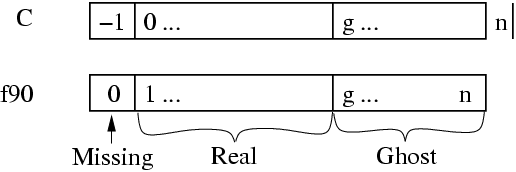
\includegraphics[width=4in]{fig/conn_indexing_old}
\end{center}
\caption{Old ghost element and node numbering.  \kw{FEM\_Get\_ghost\_*} returns $g$,
\kw{FEM\_Get\_*} returns $n$.}
\label{fig:connold}
\end{figure}



\prototype{FEM\_Get\_ghost}
\function{int FEM\_Get\_node\_ghost(void);}
\function{int FEM\_Get\_elem\_ghost(int elemType);}

The examples below iterate over the real and ghost elements using the old numbering:
\begin{alltt}
C version:
        int firstGhost,max;
        FEM\_Get\_node(\&max, \&ignored);
        firstGhost=FEM\_Get\_node\_ghost();
        for (i=0;i<firstGhost;i++)
                ... i is a real node...
        for (i=firstGhost;i<max;i++)
                ... i is a ghost node ...

Fortran version:
        call FEM\_Get\_node(max,ignored);
        firstGhost=FEM\_Get\_node\_ghost();
        do i=1,firstGhost-1
                ... i is a real node...
        end do
        do i=firstGhost,max
                ... i is a ghost node...
        end do
\end{alltt}



\subsection{Old Backward Compatability}
\prototype{FEM\_Set\_mesh}
\function{void FEM\_Set\_mesh(int nElem, int nNodes, int nodePerEl,const int* conn);}

     This is a convenience routine equivalent to:
\begin{alltt}
          FEM\_Set\_node(nNodes,0);
          FEM\_Set\_elem(0,nElem,0,nodePerEl);
          FEM\_Set\_elem\_Conn(0,conn);
\end{alltt}

\function{SUBROUTINE FEM\_Set\_mesh(nElem,nNodes,nodePerEl,conn)}
    \args{INTEGER, INTENT(IN) :: nElem, nNodes, nodePerEl}
    \args{INTEGER, INTENT(IN), dimension(nElem,nodePerEl) :: conn;}

     This is a convenience routine equivalent to:
\begin{alltt}
          CALL FEM\_Set\_node(nNodes,0)
          CALL FEM\_Set\_elem(1,nElem,0,nodePerEl)
          CALL FEM\_Set\_elem\_Conn\_c(1,conn)
\end{alltt}


\subsection{Old Sparse Data}

Sparse data is typically used to represent boundary conditions.  For
example, in a structural dynamics program typically some nodes have 
an imposed force or position.  The routines in this section are 
used to describe this kind of mesh-associated data---data that only 
applies to some ``sparse'' subset of the nodes or elements.  


\prototype{FEM\_Set\_sparse}
\function{void FEM\_Set\_sparse(int S\_id,int nRec,
         const int *nodes,int nodesPerRec,
         const void *data,int dataPerRec,int dataType);}
\function{SUBROUTINE FEM\_Set\_sparse(S\_id,nRec,nodes,nodesPerRec,data,dataPerRec,dataType)}
  \args{INTEGER, INTENT(IN) :: S\_id,nRec,nodesPerRec,dataPerRec,dataType}
  \args{INTEGER, INTENT(IN) :: nodes(nodesPerRec,nRec)}
  \args{varies,  INTENT(IN) :: data(dataPerRec,nRec)}

Register \kw{nRec} sparse data records with the framework under the number \kw{S\_id}. 
The first call to \kw{FEM\_Set\_sparse} must give a \kw{S\_id} of zero in C (1 in fortran);
and subsequent calls to \kw{FEM\_Set\_sparse} must give increasing consecutive \kw{S\_id}s.

One sparse data record consists of some number of nodes, listed in the
\kw{nodes} array, and some amount of user data, listed in the data array.
Sparse data records are copied into the chunks that contains all that record's listed 
nodes.  Sparse data records are normally used to describe mesh boundary conditions--
for node-associated boundary conditions, \kw{nodesPerRec} is 1; for triangle-associated
boundary conditions, \kw{nodesPerRec} is 3.

In general, \kw{nodePerRec} gives the number of nodes associated with each
sparse data record, and \kw{nodes} gives the actual node numbers.
\kw{dataPerRec} gives the number of data items associated with each sparse 
data record, and \kw{dataType}, one of \kw{FEM\_BYTE}, \kw{FEM\_INT},
\kw{FEM\_REAL}, or \kw{FEM\_DOUBLE}, gives the type of each data item.
As usual, you may change or delete the \kw{nodes} and \kw{data} arrays after 
this call returns.

For example, if the first set of sparse data is 17 sparse data records, each 
containing 2 nodes stored in \kw{bNodes} and 3 integers stored in \kw{bDesc}, 
we would make the call:
\begin{alltt}
/*C version*/
  FEM\_Set\_sparse(0,17, bNodes,2, bDesc,3,FEM\_INT);
! Fortran version
  CALL FEM\_Set\_sparse(1,17, bNodes,2, bDesc,3,FEM\_INT)
\end{alltt}

\prototype{FEM\_Set\_sparse\_elem}
\function{void FEM\_Set\_sparse\_elem(int S\_id,const int *rec2elem);}
\function{SUBROUTINE FEM\_Set\_sparse\_elem(S\_id,rec2elem)}
  \args{INTEGER, INTENT(IN) :: S\_id}
  \args{INTEGER, INTENT(IN) :: rec2elem(2,nRec)}

Attach the previously-set sparse records \kw{S\_id} to the given elements.
\kw{rec2elem} consists of pairs of integers---one for each sparse data record.
The first integer in the pair is the
element type to attach the sparse record to, and the second integer
gives the element number within that type.  For example, to attach
the 3 sparse records at \kw{S\_id} to the elements numbered 10, 11, and 12
of the element type \kw{elType}, use:

\begin{alltt}
/*C version*/
  int rec2elem[]={elType,10, elType,11, elType,12};
  FEM\_Set\_sparse\_elem(S\_id,rec2elem);
! Fortran version
  integer :: rec2elem(2,3);
  rec2elem(1,:)=elType
  rec2elem(2,1)=10; rec2elem(2,2)=11; rec2elem(2,3)=12;
  CALL FEM\_Set\_sparse\_elem(S\_id,rec2elem)
\end{alltt}


\prototype{FEM\_Get\_sparse}
\function{int  FEM\_Get\_sparse\_length(int S\_id);}
\function{void FEM\_Get\_sparse(int S\_id,int *nodes,void *data);}
\function{function FEM\_Get\_sparse\_length(S\_id);}
  \args{INTEGER, INTENT(IN) :: S\_id}
  \args{INTEGER, INTENT(OUT) :: FEM\_Get\_sparse\_Length}
\function{SUBROUTINE FEM\_Get\_sparse(S\_id,nodes,data);}
  \args{INTEGER, INTENT(IN) :: S\_id}
  \args{INTEGER, INTENT(OUT) :: nodes(nodesPerRec,FEM\_Get\_sparse\_Length(S\_id))}
  \args{varies,  INTENT(OUT) :: data(dataPerRec,FEM\_Get\_sparse\_Length(S\_id))}

Retrieve the previously registered sparse data from the framework.
\kw{FEM\_Get\_sparse\_length} returns the number of records of sparse
data registered under the given \kw{S\_id}; zero indicates no records
are available.  \kw{FEM\_Get\_sparse} returns you the actual nodes
(translated to local node numbers) and unchanged user data for
these sparse records.

In this old interface, there is no way to access sparse ghosts.



%%%%%%%%%%%%%%%%%%%%%%%%%%%%%%%%%%%%%%%%%%%%%%%%%%%%%%%%%%%%%%%%%%%%%%%%%%%%%%%%%%%%%%%%
\newpage
\section{Mesh Modification}


\prototype{FEM\_Update\_mesh}
\function{void FEM\_Update\_mesh(FEM\_Update\_mesh\_fn routine, int callMeshUpdated,int doWhat);}
\function{SUBROUTINE FEM\_Update\_mesh(routine,callMeshUpdated,doWhat)}
    \args{external, INTENT(IN) :: routine}
    \args{INTEGER, INTENT(IN) :: callMeshUpdated,doWhat}

Reassemble the mesh chunks from each partition into a single serial mesh,
and call the given \kw{routine} on the assembled mesh.
In this \kw{routine}, which runs on processor 0, the \kw{FEM\_Get} and \kw{FEM\_Set} routines
can manipulate the serial mesh.  The parameter \kw{callMeshUpdated}, which must
be non-zero, is passed down to \kw{routine} as \kw{routine(callMeshUpdated)}.

\kw{FEM\_Get} calls from
\kw{driver()} will only return the new mesh after a \kw{FEM\_Update\_mesh} call
where \kw{doWhat} is \kw{FEM\_MESH\_UPDATE}; otherwise \kw{FEM\_Get} from \kw{driver()} will still
return the old mesh.
\kw{FEM\_Update\_mesh} can only be called from driver; and must be called by the driver routine for
every chunk. 

%     If \kw{doRepartition} is 0, the mesh is not repartitioned, and \kw{FEM\_Update\_mesh}
%returns immediately.  If \kw{doRepartition} is 1, \kw{FEM\_Update\_mesh} blocks
%until the reassembled serial mesh is repartitioned back into chunks and redistributed.
%If \kw{doRepartition} is 2, 

\begin{center}
\begin{tabular}{|l|l|l|l|}\hline
\kw{doWhat} & Numeric & Repartition? & \kw{FEM\_Update\_mesh} \\\hline
\kw{FEM\_MESH\_OUTPUT} & 0 & No & \kw{driver()} continues alongside \kw{routine} \\
\kw{FEM\_MESH\_FINALIZE} & 2 & No & \kw{driver()} blocks until \kw{routine} finishes\\
\kw{FEM\_MESH\_UPDATE} & 1 & Yes & \kw{driver()} blocks for the new partition \\
\hline
\end{tabular}
\end{center}

For example, \kw{FEM\_Update\_mesh}(\uw{my\_output\_routine}, \uw{k}, \kw{FEM\_MESH\_OUTPUT}) 
reassembles the mesh and calls a routine named
\uw{my\_output\_routine(k)} while the driver routines continue with the computation.
This might be useful, for example, for writing out intermediate solutions as a 
single file; writing outputs from \kw{driver()} is more efficient but often results 
in a separate file for each mesh chunk.

   To block the driver routines during a call to a routine named
\uw{my\_finalize\_routine(k)}, such as 
at the end of the computation when the drivers have no other work to do, 
use \kw{FEM\_Update\_mesh}(\uw{my\_finalize\_routine}, \uw{k}, \kw{FEM\_MESH\_FINALIZE}).

     To reassemble, modify, and repartition the mesh, use
\kw{FEM\_Update\_mesh}(\uw{my\_update\_routine}, \uw{k}, \kw{FEM\_MESH\_UPDATE}).
It may be easier to perform major mesh modifications from \uw{my\_update\_routine(k)} than
the drivers, since the entire serial mesh is available to \uw{my\_update\_routine(k)}.

     \kw{FEM\_Update\_mesh} reassembles the serial mesh with an attempt to
     preserve the element and node global numbering.  If the new mesh
     has the same number and type of elements and nodes, the global
     numbers (and hence serial mesh) will be unchanged.  If new
     elements or nodes are added at each chunk, they will be assigned
     new unique global numbers.  If elements or nodes are removed,
     their global numbers are not re-used-- you can detect the
     resulting holes in the serial mesh since the user data associated
     with the deleted elements will be all zero.  Generally, however, it
     is less error-prone to perform mesh modifications only in \kw{driver()}
     or only in an update routine, rather than some in both.


